\documentclass[10pt,letterpaper]{article}

\usepackage[margin=0.74in,top=0.75in,bottom=0.76in]{geometry}
\usepackage{fontspec}
\setmainfont{Charter}
\setsansfont{Helvetica Neue}
\setmonofont[Scale=0.84]{Menlo}

\usepackage{microtype}
\usepackage{xcolor}
\usepackage{booktabs}
\usepackage{tabularx}
\usepackage{array}
\usepackage{enumitem}
\usepackage{titlesec}
\usepackage{fancyhdr}
\usepackage[most]{tcolorbox}
\usepackage{tikz}
\usetikzlibrary{arrows.meta,positioning,fit,shapes.geometric,calc}
\usepackage{pgfplots}
\pgfplotsset{compat=1.18}
\usepackage{lastpage}
\usepackage{hyperref}

% Palette
\definecolor{InkNavy}{HTML}{16243E}
\definecolor{SlateBlue}{HTML}{2B5B84}
\definecolor{ForestTeal}{HTML}{0F766E}
\definecolor{WarmAmber}{HTML}{B45309}
\definecolor{CrimsonMute}{HTML}{991B1B}
\definecolor{SoftBg}{HTML}{F4F7FA}
\definecolor{WarmBg}{HTML}{FFFBEB}
\definecolor{TealBg}{HTML}{F0FDFA}
\definecolor{RuleGray}{HTML}{CBD5E1}
\definecolor{MutedGray}{HTML}{475569}

\hypersetup{
  colorlinks=true,
  linkcolor=SlateBlue,
  urlcolor=SlateBlue,
  citecolor=SlateBlue,
  pdftitle={Agentic File System (AFS): Research Lineage, Repository Evolution, and Empirical Telemetry},
  pdfauthor={Justin Scofield},
  pdfsubject={Agentic File System, Context Engineering, 490-Commit Evolution, and Harness Research}
}

% Typography & spacing
\setlength{\parindent}{0pt}
\setlength{\parskip}{4.5pt}
\setlength{\emergencystretch}{1.8em}
\renewcommand{\arraystretch}{1.15}
\setlist[itemize]{leftmargin=1.35em, itemsep=2.0pt, topsep=2.2pt, parsep=0pt}
\setlist[enumerate]{leftmargin=1.5em, itemsep=2.0pt, topsep=2.2pt, parsep=0pt}

% Headings
\titleformat{\section}
  {\sffamily\bfseries\large\color{InkNavy}}
  {\thesection.}{0.55em}{}[\vspace{2pt}{\color{RuleGray}\titlerule[0.6pt]}]
\titlespacing*{\section}{0pt}{12pt}{5pt}

\titleformat{\subsection}
  {\sffamily\bfseries\normalsize\color{SlateBlue}}
  {\thesubsection}{0.5em}{}
\titlespacing*{\subsection}{0pt}{8pt}{3pt}

% Running headers / footers
\pagestyle{fancy}
\fancyhf{}
\fancyhead[L]{\sffamily\footnotesize\color{MutedGray} Agentic File System (AFS): Research Lineage, Evolution \& Telemetry}
\fancyhead[R]{\sffamily\footnotesize\color{MutedGray} Technical Whitepaper \textbullet\ November 2026}
\fancyfoot[C]{\sffamily\footnotesize\color{MutedGray} Page \thepage\ of \pageref{LastPage}}
\renewcommand{\headrulewidth}{0.4pt}
\renewcommand{\footrulewidth}{0pt}

% Boxes
\newtcolorbox{summarybox}[1]{
  colback=SoftBg,
  colframe=SlateBlue,
  boxrule=0.7pt,
  arc=3pt,
  left=10pt, right=10pt, top=7pt, bottom=7pt,
  fonttitle=\sffamily\bfseries\small\color{white},
  coltitle=white,
  colbacktitle=InkNavy,
  title={#1}
}

\newtcolorbox{auditbox}[1]{
  colback=WarmBg,
  colframe=WarmAmber,
  boxrule=0.7pt,
  arc=3pt,
  left=10pt, right=10pt, top=7pt, bottom=7pt,
  fonttitle=\sffamily\bfseries\small\color{white},
  coltitle=white,
  colbacktitle=WarmAmber,
  title={#1}
}

\newtcolorbox{tealbox}[1]{
  colback=TealBg,
  colframe=ForestTeal,
  boxrule=0.7pt,
  arc=3pt,
  left=10pt, right=10pt, top=7pt, bottom=7pt,
  fonttitle=\sffamily\bfseries\small\color{white},
  coltitle=white,
  colbacktitle=ForestTeal,
  title={#1}
}

\newcommand{\code}[1]{\texttt{\color{InkNavy}#1}}
\newcommand{\home}{\code{\textasciitilde}}
\newcommand{\arxiv}[1]{\href{https://arxiv.org/abs/#1}{\code{arXiv:#1}}}
\newcommand{\badge}[2]{\textcolor{#1}{\sffamily\bfseries\scriptsize #2}}

\begin{document}

% Header Banner
\begin{center}
  {\sffamily\bfseries\LARGE\color{InkNavy} Agentic File System (AFS):\\[2pt] Research Lineage, Repository Evolution, and Empirical Telemetry}\\[6pt]
  {\sffamily\normalsize\color{SlateBlue} Tracing AFS from \emph{``Everything is Context''} Across 490 Commits, 583K Archived Events, and 2026 Harness Science}\\[5pt]
  {\sffamily\small\color{MutedGray} Justin Scofield \quad\textbar\quad Technical Retrospective \& Architectural Analysis \quad\textbar\quad November 26, 2026}
\end{center}
\vspace{2pt}

\begin{summarybox}{Executive Summary}
The \textbf{Agentic File System (AFS)} is an independent, harness-neutral implementation and extension of the filesystem abstraction introduced by Xu et al.\ (Dec 5, 2025, \arxiv{2512.05470}), \emph{``Everything is Context: Agentic File System Abstraction for Context Engineering''} [1]. Downloaded four days after publication alongside companion papers on agent scaling [2], single-tool code navigation [3], monadic context flow [4], infinite-horizon file state [5], and human--AI synergy [6], the blueprint became a working context-panel prototype on Dec 10, 2025 and the standalone \code{afs} repository (\code{3574cb8}) on Dec 30, 2025, building atop pre-paper context logs dating to Oct 13, 2025.

Across \textbf{490 commits} and \textbf{583,016 archived events} spanning 14 months (\code{560} unique log files), AFS evolved through full expansion (peaking at \textbf{350 modules / 136.4k LOC} in Sep 2026), deliberate \emph{afs-lite} contraction (\textbf{300 modules / 126.7k LOC}, \textbf{200 test modules}, and a \textbf{16-tool frozen slim MCP catalog}), and November 2026 cryptographic gate hardening. Archived telemetry directly corroborates minimal-scaffold theory: out of \textbf{70,063 MCP tool calls} (98.4\% success rate), just \textbf{five tools drive 97.2\%} of all usage; \textbf{27,085 CLI invocations} center on \code{session bootstrap} (9,744 runs); and \textbf{8,715 Hivemind messages} across six active roots demonstrate a $3.0\times$ multi-agent acceleration between October and November 2026. Evaluated against 34 source and validation studies, AFS emerges as an \emph{extended cognition} OS built and battle-tested ahead of the 2026 harness-engineering wave.
\end{summarybox}

\section{Direct Inspirations: The Primary Reading Corpus (Dec 2025 -- Jan 2026)}

\begin{sloppypar}
Reconstructing AFS's actual intellectual lineage from \code{docs/LINEAGE.md}, historical git snapshots (\code{docs/RESEARCH\_SOURCES.md}, \code{docs/NARRATIVE.md}, \code{docs/CLI\_PLAN.md}, \code{docs/RESEARCH\_INFIAGENT.md}), and the local \home\code{/Documents/Research/} library reveals a specific founding design cluster quite distinct from generic retrofitted citations.
\end{sloppypar}

\subsection{\texorpdfstring{Primary Blueprint: \emph{``Everything is Context''} (\arxiv{2512.05470})}{Primary Blueprint: Everything is Context (arXiv:2512.05470)}}
Xu et al.\ [1] framed context engineering around Unix's ``everything is a file'' abstraction --- replacing ad-hoc prompt gluing and fragmented RAG with a persistent, governed filesystem hierarchy processed through a Context Constructor, Loader/Updater, and Evaluator inside ArcBlock's TypeScript \emph{AIGNE} framework. AFS is an independent Python realization unaffiliated with CSIRO Data61 or ArcBlock. Table~\ref{tab:xu_map} summarizes the direct mapping and AFS's seven original extensions beyond the paper.

\begin{table}[ht!]
\centering
\sffamily\footnotesize
\begin{tabularx}{\textwidth}{@{}>{\raggedright\bfseries\arraybackslash}p{3.0cm} >{\raggedright\arraybackslash}p{5.8cm} >{\raggedright\arraybackslash}X@{}}
\toprule
\color{InkNavy}Paper Concept [1] & \color{InkNavy}AFS Core Realization & \color{InkNavy}AFS Original Extensions Beyond Paper \\
\midrule
Typed Uniform Mounts &
V1 role mounts; opt-in V2 6 categories (\code{history}, \code{memory}, \code{scratchpad}, \code{knowledge}, \code{tools}, \code{human}) + internal \code{.afs/}. &
\textbf{Harness Neutrality:} Decouples \code{.context/} from any single framework so Claude, Codex, Gemini (\code{gemini-cli} $\rightarrow$ Antigravity \code{agy}), and Cursor share state. \\
\addlinespace[2.5pt]
Persistent Repository &
Markdown files + rebuildable SQLite FTS5 \& opt-in vector indexes (\code{context\_index.py}). &
\textbf{Central Scoped V2:} Stable \code{prj\_<uuid>} scopes, default current+common reads, atomic \code{renamex\_np} migration/rollback. \\
\addlinespace[2.5pt]
History / Memory / Scratchpad &
Append-only JSONL/gzip logs; memory consolidation (\code{memory\_consolidation.py}); draft notes with promotion. &
\textbf{Immutable Revision Handoffs:} Chained \code{supersedes} Markdown handoffs + \textbf{Multi-Agent Bus} (\code{messages.sqlite3} + \code{message\_doorbell.py}). \\
\addlinespace[2.5pt]
Constructor / Loader &
Token-budgeted \code{context\_pack.py} (RRF retrieval); \code{session\_bootstrap.py} and client wrappers. &
\textbf{Operational Layer:} \code{afs doctor}, \code{afs history reap}, \code{storage audit}, and event reactor. \\
\addlinespace[2.5pt]
Evaluator / Human Input &
Schema checks (\code{schema.py}), execution broker, pure \code{optimize decide}; controlling-terminal \code{approvals}. &
\textbf{Engagement Primitives:} \code{HumanDecisionBroker}, mandatory \code{--because}, calibration scoring, and unforgeable \code{human\_intent}. \\
\bottomrule
\end{tabularx}
\caption{Mapping Xu et al.'s \emph{Everything is Context} [1] onto AFS core primitives and original engineering extensions (per \code{docs/LINEAGE.md}).}
\label{tab:xu_map}
\end{table}

\subsection{\texorpdfstring{Companion Papers Cataloged in Repo History \& \home\code{/Documents/Research/}}{Companion Papers Cataloged in Repo History and ~/Documents/Research/}}
Alongside \arxiv{2512.05470}, AFS's historical catalog documents how seven distinct technical threads downloaded in Dec 2025 -- Jan 2026 shaped specific design decisions:

\begin{table}[ht!]
\centering
\sffamily\footnotesize
\begin{tabularx}{\textwidth}{@{}>{\raggedright\bfseries\arraybackslash}p{3.9cm} >{\raggedright\arraybackslash}p{4.3cm} >{\raggedright\arraybackslash}X@{}}
\toprule
\color{InkNavy}Primary Source (Local Date) & \color{InkNavy}Core Thesis & \color{InkNavy}Direct Architectural Influence on AFS \\
\midrule
Xu et al.\ \arxiv{2512.05470} [1] (Dec 9, 2025) &
Unix file-system abstraction for persistent context engineering. &
Adopted within 24h (Dec 10 prototype $\rightarrow$ Dec 30 repo baseline \code{3574cb8}); canonical cite in \code{LINEAGE.md} \& \code{NARRATIVE.md}. \\
\addlinespace[2.5pt]
Riedl \& Weidmann [6] (Dec 9, 2025) &
Bayesian IRT quantifying human--AI synergy \& Theory of Mind over raw model accuracy. &
Framed human checkpoints and cognitive telemetry around joint human--AI ability rather than zero-touch autonomy (\code{NARRATIVE.md}). \\
\addlinespace[2.5pt]
Kim et al.\ \arxiv{2512.08296} [2] (Dec 11, 2025) &
Quantitative scaling principles, coordination trade-offs, and tool overhead in multi-agent systems. &
Motivated \code{CLI\_PLAN.md} observability hooks, structured run metrics, and later Hivemind broker boundaries. \\
\addlinespace[2.5pt]
Zhang et al.\ \arxiv{2512.20957} [3] (Dec 30, 2025) &
\emph{One Tool Is Enough} (RepoNavigator): execution-aware minimal tool beat multi-tool bloat. &
Directly drove \code{CLI\_PLAN.md}'s minimal tool surface principle and foreshadowed the 16-tool slim MCP freeze. \\
\addlinespace[2.5pt]
Zhang \& Wang \arxiv{2512.22431} [4] (Dec 30, 2025) &
\emph{Monadic Context Engineering}: explicit algebraic composition of state, errors, and async effects. &
Shaped explicit context-flow and failure-boundary contracts in \code{CLI\_PLAN.md}, \code{execution/}, and atomic migration. \\
\addlinespace[2.5pt]
Yu et al.\ \arxiv{2601.03204} [5] (Jan 10, 2026) &
\emph{InfiAgent}: File-centric state $S_t = F_t$ keeps working context $O(1)$; \emph{External Attention} isolates doc reads. &
Analyzed in \code{RESEARCH\_INFIAGENT.md}; validated ``Context as Files,'' state refresh consolidation, and alpha/domain hierarchy. \\
\addlinespace[2.5pt]
Guo et al.\ [7], Marek et al.\ [8], Dobariya \& Kumar [9] &
\emph{SonicMoE}, \emph{Small Batch Size Training}, and \emph{Mind Your Tone} terse prompt behavior. &
Guided Jan 2026 in-tree training/MoE exploration (later moved cleanly to \code{afs-scawful}) and clipped, non-theatrical prompts. \\
\addlinespace[2.5pt]
Google DevProd \& Code-Review Corpus [10--16] (Dec 11--12, 2025) &
Empirical Google studies on code metadata [10], practice checks [11], ML review fixes [12], productivity [13--15], mutants [16]. &
Shaped AFS's practitioner focus on code-review friction, structured verification evidence, and developer velocity metrics. \\
\bottomrule
\end{tabularx}
\caption{Primary source corpus verified in \home\code{/Documents/Research/} and AFS git commits (\code{b28c092}, \code{b0f51f39}, \code{39561d7\textasciitilde1}).}
\label{tab:corpus}
\end{table}

\begin{figure}[ht!]
\centering
\resizebox{\textwidth}{!}{%
\begin{tikzpicture}[
  font=\sffamily\scriptsize,
  >=Stealth,
  box/.style={draw=InkNavy!75, rounded corners=3pt, fill=white, align=center, minimum height=0.90cm, inner xsep=6pt, inner ysep=4pt},
  accent/.style={draw=ForestTeal!85, thick, rounded corners=3pt, fill=TealBg, align=center, minimum height=0.90cm, inner xsep=6pt, inner ysep=4pt},
  warn/.style={draw=WarmAmber!85, thick, rounded corners=3pt, fill=WarmBg, align=center, minimum height=0.90cm, inner xsep=6pt, inner ysep=4pt},
  note/.style={font=\sffamily\scriptsize\color{MutedGray}, align=left, anchor=west}
]

% Layer 1: Clients & Surfaces
\node[box, text width=3.4cm] (cli) at (0.0, 3.25) {\textbf{Host CLIs}\\Claude / Codex / Gemini (\code{agy})\\{\tiny\color{MutedGray}(migrated from \code{gemini-cli})}};
\node[box, text width=3.6cm] (mcp) at (4.4, 3.25) {\textbf{Frozen Slim MCP}\\16 tools (vs.\ 106 full) [3, 24]};
\node[box, text width=3.8cm] (barista) at (9.0, 3.25) {\textbf{Barista Files \& Mobile}\\Pocket Hub HTTP + SSE};

% Layer 2: Control & Runtime Primitives
\node[accent, text width=3.4cm] (pack) at (0.1, 1.50) {\textbf{Session \& Context Pack}\\\code{--short} / RRF / FTS5 [1, 5, 20]};
\node[warn, text width=3.9cm] (gate) at (4.55, 1.50) {\textbf{ApprovalGate v2}\\Audit + SHA-256 [26, 32, 33]};
\node[accent, text width=3.5cm] (bus) at (9.1, 1.50) {\textbf{Hivemind + Doorbell}\\Hooks + Thread Ring [2, 22]};

% Layer 3: Durable Persistence
\node[box, text width=5.1cm, minimum height=0.96cm] (md) at (1.35, -0.30) {\textbf{Markdown Sources of Truth}\\\code{scratchpad/} \textbullet\ \code{memory/} \textbullet\ \code{knowledge/} [1, 5]};
\node[box, text width=5.7cm, minimum height=0.96cm] (db) at (7.85, -0.30) {\textbf{SQLite WAL Stores} (\code{user\_version} migrations)\\\code{approvals} \textbullet\ \code{messages} \textbullet\ \code{context\_index}};

% Arrows
\draw[->, thick, SlateBlue] (cli.south) -- (pack.north);
\draw[->, thick, SlateBlue] ($(mcp.south)+(-0.6,0)$) -- ($(pack.north)+(0.6,0)$);
\draw[->, thick, SlateBlue] (mcp.south) -- (gate.north);
\draw[->, thick, SlateBlue] (barista.south) -- (bus.north);
\draw[->, thick, SlateBlue] ($(cli.south)+(0.9,0)$) -- ($(gate.north)+(-1.1,0)$);
\draw[->, thick, ForestTeal] (pack.south) -- ($(md.north)+(-0.4,0)$);
\draw[->, thick, ForestTeal] ($(pack.south)+(0.8,0)$) -- ($(db.north)+(-1.9,0)$);
\draw[->, thick, WarmAmber] (gate.south) -- ($(db.north)+(-0.5,0)$);
\draw[->, thick, ForestTeal] (bus.south) -- ($(db.north)+(1.2,0)$);

% Labels on right
\node[note] at (11.75, 3.25) {\textbf{Surface Tier}\\Harness-Neutral Client Bus};
\node[note] at (11.75, 1.50) {\textbf{Control Tier}\\Calibrated Human Synergy [6]};
\node[note] at (11.75, -0.30) {\textbf{State Tier}\\Context-as-Files OS [1, 25]};

\end{tikzpicture}%
}
\caption{AFS three-layer runtime architecture mapping external harnesses to core primitives and durable state, integrating primary inspirations [1--6] and 2026 security hardening [26, 32, 33].}
\label{fig:arch}
\end{figure}

\section{490-Commit Repository Evolution (Dec 2025 -- Nov 2026)}

Walking the entire \code{afs} commit graph (\code{3574cb8} on Dec 30, 2025 through \code{54150e5} plus Nov 25--26 hardening) explains why the repository looks the way it does today: it underwent an intentional \emph{expand, separate, harden, and contract} lifecycle rather than unchecked bloat.

\begin{table}[ht!]
\centering
\sffamily\footnotesize
\begin{tabularx}{\textwidth}{@{}>{\raggedright\bfseries\arraybackslash}p{2.7cm} >{\raggedright\arraybackslash}p{2.6cm} >{\raggedright\arraybackslash}X@{}}
\toprule
\color{InkNavy}Architectural Era & \color{InkNavy}Scale (\code{src/afs}) & \color{InkNavy}Key Commits \& Structural Transitions \\
\midrule
1. Precursor \& Baseline (Oct 2025 -- Jan 2026, 70 commits) &
$21 \rightarrow 202$ modules; $3.1\text{k} \rightarrow 62.9\text{k}$ LOC; $7 \rightarrow 34$ tests &
Pre-repo context logs start Oct 13, 2025; Dec 10 prototype; \code{3574cb8} baseline (Dec 30) + AFS Studio (\code{5db5f87}) + research catalog (\code{b28c092}). Jan explodes outward with training generators, synthetic data, discriminator, and MoE exploration. \\
\addlinespace[2.5pt]
2. Extension Split \& \code{gemini-cli} MCP (Mar -- Apr 2026, 120 commits) &
$205 \rightarrow 298$ modules; $63.6\text{k} \rightarrow 90.7\text{k}$ LOC; $35 \rightarrow 124$ tests &
Moves domain/training/MoE behind \code{afs-scawful} (\code{6db8053}, \code{51dace6}), scrubs personal refs (\code{abb4278}, \code{39561d7}), introduces MCP (\code{eee5e1f}), SQLite index (\code{fb12425}), VS Code (\code{5e57f2c}), heavy \code{gemini-cli} integration (\code{56ef9a5}, \code{814dd0b}, \code{cf904b3}), and early Antigravity config (\code{d587e3f}). \\
\addlinespace[2.5pt]
3. Trust Boundaries \& Layout v2 (Jun -- Jul 2026, 223 commits, \code{v0.2.0}) &
$313 \rightarrow 332$ modules; $94.8\text{k} \rightarrow 131.3\text{k}$ LOC; $129 \rightarrow 178$ tests &
Adds Antigravity adapter (\code{c766949}); peaks in July (44\% of repo commits): \code{LINEAGE.md} (\code{96d9fbf}), \textbf{Engagement Primitives} (\code{d199ca8}: \code{--because}, calibration, \code{human\_intent}), Execution Broker (\code{951e19a}), pure Optimization Gate (\code{233520f}), Event Reactor (\code{a9351b1}), Bounded Skills (\code{8cf925a}), Layout v2 atomic cutover (\code{a6853d0}, \code{3db89f4}), Storage Audit (\code{c1b7545}). \\
\addlinespace[2.5pt]
4. Peak \& \emph{afs-lite} / \code{agy} (Sep -- Nov 2026, 69 commits) &
Peak $350$ modules / $136.4\text{k}$ LOC (Sep) $\rightarrow 300$ / $126.7\text{k}$ (Nov); $200$ tests &
\code{RETOOL\_PLAN.md} executes deliberate subtraction: drops $\sim 13.8\text{k}$ LOC of dead packages (\code{bb125db}, \code{7f2d23c}), freezes 16-tool slim MCP (\code{df41ff8}), migrates approvals \& mail to SQLite (\code{0fd03bb}, \code{6c765a7}), gates training/embeddings (\code{bc59985}), adds \code{history reap} (\code{fbb2593}), Antigravity (\code{agy}) doorbell wakes, and v2 Loopjacking + Audit hardening (Nov 25). \\
\bottomrule
\end{tabularx}
\caption{Four-era trajectory across all 490 commits of \code{scawful/afs} measured from monthly git tree snapshots.}
\label{tab:git_eras}
\end{table}

\textbf{Empirical Proof of Harness Neutrality (Gemini: \code{gemini-cli} $\rightarrow$ Antigravity \code{agy}).} Heavy Gemini workflows initially ran through \code{gemini-cli} (\code{afs gemini}, cached content \code{814dd0b}, workspace wrappers \code{cf904b3}) from late 2025 through April 2026 before migrating to \textbf{Antigravity (\code{agy})} (\code{afs antigravity}, shared \code{.agents/skills/}, and detached \code{ring\_agy()} doorbell wakeups in Nov 2026) once \code{gemini-cli} was deprecated. Because \code{.context/} knowledge, FTS5 indexes, and handoff state live outside any vendor harness, the runtime switch preserved full session continuity without re-engineering context plumbing.

\begin{figure}[ht!]
\centering
\resizebox{\textwidth}{!}{%
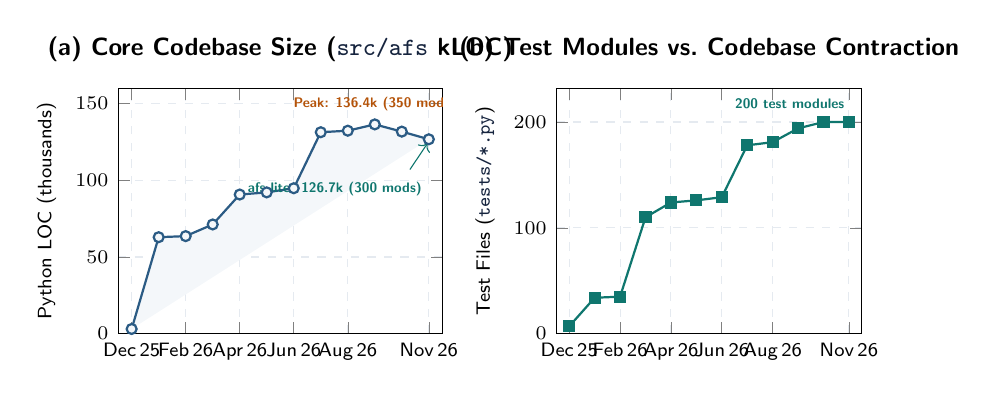
\begin{tikzpicture}
\begin{axis}[
  name=locplot,
  width=0.47\textwidth,
  height=4.7cm,
  title={\sffamily\bfseries\small (a) Core Codebase Size (\code{src/afs} kLOC)},
  ylabel={\sffamily\scriptsize Python LOC (thousands)},
  xmin=0.5, xmax=12.5,
  ymin=0, ymax=160,
  xtick={1,3,5,7,9,12},
  xticklabels={Dec\,25, Feb\,26, Apr\,26, Jun\,26, Aug\,26, Nov\,26},
  tick label style={font=\sffamily\scriptsize},
  grid=major,
  major grid style={RuleGray!50, dashed}
]
\addplot[color=SlateBlue, thick, mark=*, mark size=1.8pt, fill=SoftBg] coordinates {
  (1,3.1) (2,62.9) (3,63.6) (4,71.2) (5,90.7) (6,92.1) (7,94.8) (8,131.3) (9,132.3) (10,136.4) (11,131.7) (12,126.7)
};
\node[font=\sffamily\tiny\color{WarmAmber}, anchor=south] at (axis cs:10,139) {\textbf{Peak: 136.4k (350 mods)}};
\node[font=\sffamily\tiny\color{ForestTeal}, anchor=north east] at (axis cs:12.1,105) {\textbf{afs-lite: 126.7k (300 mods)}};
\draw[->, thin, ForestTeal] (axis cs:11.3,107) -- (axis cs:11.95,124);
\end{axis}

\begin{axis}[
  at={(locplot.south east)},
  anchor=south west,
  xshift=1.45cm,
  width=0.45\textwidth,
  height=4.7cm,
  title={\sffamily\bfseries\small (b) Test Modules vs.\ Codebase Contraction},
  ylabel={\sffamily\scriptsize Test Files (\code{tests/*.py})},
  xmin=0.5, xmax=12.5,
  ymin=0, ymax=232,
  xtick={1,3,5,7,9,12},
  xticklabels={Dec\,25, Feb\,26, Apr\,26, Jun\,26, Aug\,26, Nov\,26},
  tick label style={font=\sffamily\scriptsize},
  grid=major,
  major grid style={RuleGray!50, dashed}
]
\addplot[color=ForestTeal, thick, mark=square*, mark size=1.8pt] coordinates {
  (1,7) (2,34) (3,35) (4,110) (5,124) (6,126) (7,129) (8,178) (9,181) (10,194) (11,200) (12,200)
};
\node[font=\sffamily\tiny\color{ForestTeal}, anchor=south east] at (axis cs:12.2,204) {\textbf{200 test modules}};
\end{axis}
\end{tikzpicture}%
}
\caption{Monthly \code{src/afs} LOC and \code{tests/} module counts reconstructed from git snapshots (\code{6729409} through \code{54150e5}). Test density increased steadily even as \emph{afs-lite} cut 50 production modules ($-9.7\text{k}$ LOC) between Sep and Nov 2026.}
\label{fig:git_evolution}
\end{figure}

\section{Longitudinal Production Telemetry (583,016 Archived Events)}

Deduplicating symlinks across seven active and archived workspace history stores yields \textbf{560 unique \code{.jsonl} / \code{.jsonl.gz} files} spanning Oct 13, 2025 through Nov 25, 2026, totaling \textbf{583,016 logged events} alongside \textbf{8,715 Hivemind SQLite messages}. These archives expose four empirical patterns directly relevant to harness research:

\begin{enumerate}
  \item \textbf{Extreme Pareto Tool Concentration (\code{mcp\_tool}: 70,063 calls, 98.4\% ok):} Out of 106 catalog tools, only \textbf{42} were ever called. Two primitives --- \code{context.read} (25,975 calls; 37.1\%) and \code{context.write} (25,936 calls; 37.0\%) --- account for \textbf{74.1\%} of all MCP invocations. Adding SQLite mail (\code{messages.send} 6,783; \code{messages.read} 5,353; \code{messages.ack} 4,041) raises cumulative coverage to \textbf{97.2\%} with just five tools; the Top 10 capture \textbf{99.5\%}. This production distribution empirically vindicates Zhang et al.'s minimal-tool finding [3] and Sakizli's schema-compression imperative [24].
  \item \textbf{Warm-Start CLI Dominance (\code{cli}: 27,085 calls):} \code{session bootstrap} alone accounts for \textbf{9,744 invocations} (36.0\%), followed by \code{fs write} (4,026), \code{messages list} (3,182), \code{fs read} (2,328), \code{messages send} (1,973), and \code{messages ack} (1,796) --- together representing \textbf{85.1\%} of all CLI usage.
  \item \textbf{Supervisor Spawns \& Non-Rubber-Stamp Human Gates (\code{agent\_lifecycle}: 393,615 events):} Archived runs record \textbf{197,417 agent spawns} and \textbf{182,909 completions} (92.7\% completion, 6.0\% failure), plus \textbf{600 explicit review gates} resolving to \textbf{150 approved} and \textbf{150 rejected} --- an exact 50\%/50\% discrimination split showing real human filtering rather than automatic rubber-stamping.
  \item \textbf{Multi-Agent Swarm Surge in Oct--Nov 2026 (8,715 SQLite Hivemind messages):} Cross-agent messaging jumped \textbf{3.0$\times$} from October (2,182 messages) to November (6,531 messages), dominated by \code{status} (4,136), \code{request} (1,278), \code{handoff} (629), \code{result} (532), \code{claim} (306), and \code{review} (246) across 437 tracked Codex (279) and Claude (158) sessions.
\end{enumerate}

\begin{figure}[ht!]
\centering
\resizebox{\textwidth}{!}{%
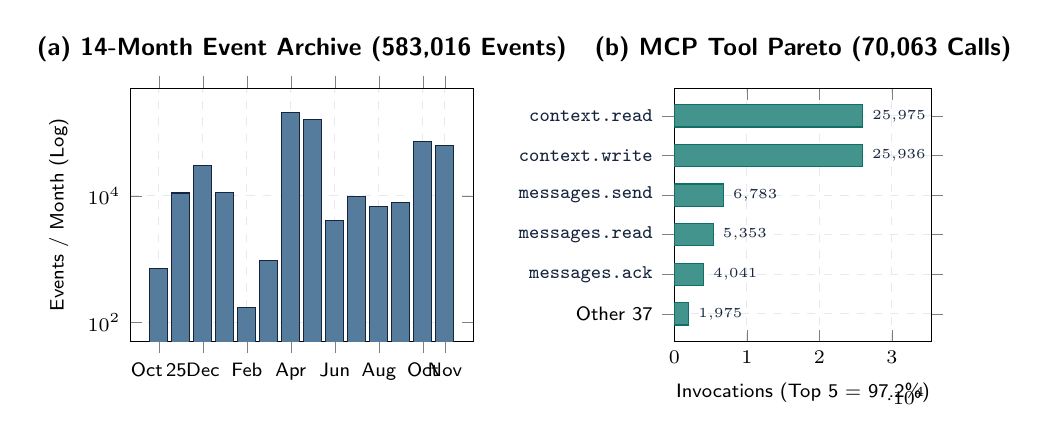
\begin{tikzpicture}
\begin{axis}[
  name=histplot,
  ybar,
  width=0.49\textwidth,
  height=4.8cm,
  ymode=log,
  ymin=50, ymax=500000,
  bar width=6.5pt,
  title={\sffamily\bfseries\small (a) 14-Month Event Archive (583,016 Events)},
  ylabel={\sffamily\scriptsize Events / Month (Log)},
  symbolic x coords={25-10, 25-11, 25-12, 26-01, 26-02, 26-03, 26-04, 26-05, 26-06, 26-07, 26-08, 26-09, 26-10, 26-11},
  xtick={25-10, 25-12, 26-02, 26-04, 26-06, 26-08, 26-10, 26-11},
  xticklabels={Oct\,25, Dec, Feb, Apr, Jun, Aug, Oct, Nov},
  tick label style={font=\sffamily\scriptsize},
  grid=major,
  major grid style={RuleGray!50, dashed}
]
\addplot[fill=SlateBlue!80, draw=InkNavy] coordinates {
  (25-10,711) (25-11,11094) (25-12,30508) (26-01,11327) (26-02,170) (26-03,947)
  (26-04,204895) (26-05,159991) (26-06,4057) (26-07,9737) (26-08,6803) (26-09,7816)
  (26-10,73036) (26-11,61924)
};
\end{axis}

\begin{axis}[
  at={(histplot.south east)},
  anchor=south west,
  xshift=2.55cm,
  xbar,
  width=0.40\textwidth,
  height=4.8cm,
  xmin=0, xmax=35500,
  enlarge y limits=0.14,
  bar width=8pt,
  title={\sffamily\bfseries\small (b) MCP Tool Pareto (70,063 Calls)},
  xlabel={\sffamily\scriptsize Invocations (Top 5 = 97.2\%)},
  symbolic y coords={other, m_ack, m_read, m_send, c_write, c_read},
  yticklabels={Other 37, \code{messages.ack}, \code{messages.read}, \code{messages.send}, \code{context.write}, \code{context.read}},
  ytick=data,
  tick label style={font=\sffamily\scriptsize},
  nodes near coords,
  nodes near coords align={horizontal},
  every node near coord/.append style={font=\sffamily\tiny\color{InkNavy}},
  grid=major,
  major grid style={RuleGray!50, dashed}
]
\addplot[fill=ForestTeal!78, draw=ForestTeal!95!black] coordinates {
  (1975,other) (4041,m_ack) (5353,m_read) (6783,m_send) (25936,c_write) (25975,c_read)
};
\end{axis}
\end{tikzpicture}%
}
\caption{Longitudinal event archive across 560 deduplicated history files (\textbf{583,016 events}) and extreme MCP Pareto concentration (\textbf{97.2\%} in five primitives, validating \emph{afs-lite}'s 16-tool slim catalog freeze).}
\label{fig:archive_pareto}
\end{figure}

\begin{figure}[ht!]
\centering
\resizebox{\textwidth}{!}{%
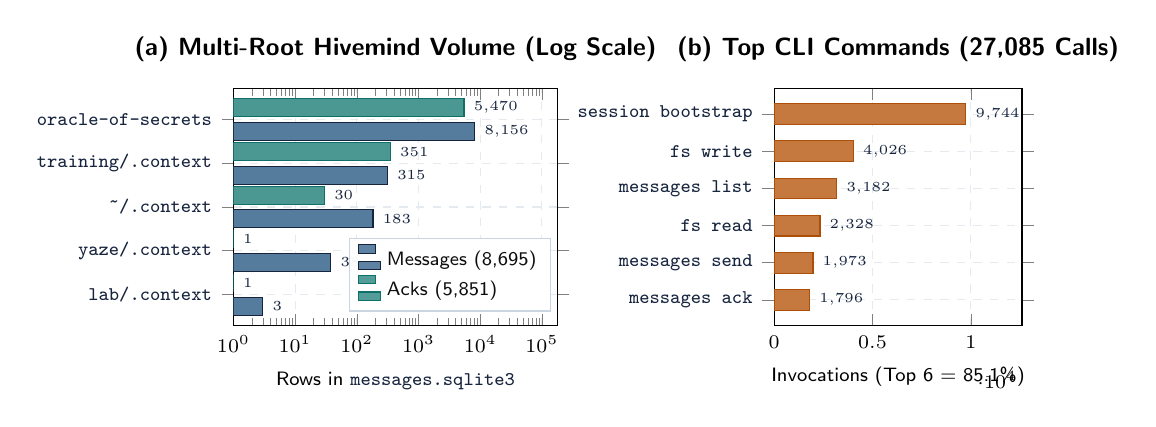
\begin{tikzpicture}
\begin{axis}[
  name=busplot,
  xbar,
  width=0.47\textwidth,
  height=4.6cm,
  xmode=log,
  xmin=1, xmax=180000,
  enlarge y limits=0.18,
  bar width=6.5pt,
  title={\sffamily\bfseries\small (a) Multi-Root Hivemind Volume (Log Scale)},
  xlabel={\sffamily\scriptsize Rows in \code{messages.sqlite3}},
  symbolic y coords={lab, yaze, home, training, oracle},
  yticklabels={\code{lab/.context}, \code{yaze/.context}, \home\code{/.context}, \code{training/.context}, \code{oracle-of-secrets}},
  ytick=data,
  tick label style={font=\sffamily\scriptsize},
  legend style={at={(0.98,0.06)}, anchor=south east, font=\sffamily\scriptsize, draw=RuleGray, fill=white, fill opacity=0.95, cells={anchor=west}},
  nodes near coords,
  nodes near coords align={horizontal},
  every node near coord/.append style={font=\sffamily\tiny\color{InkNavy}},
  point meta=rawx,
  grid=major,
  major grid style={RuleGray!50, dashed}
]
\addplot[fill=SlateBlue!80, draw=InkNavy] coordinates {
  (3,lab) (38,yaze) (183,home) (315,training) (8156,oracle)
};
\addplot[fill=ForestTeal!75, draw=ForestTeal!95!black] coordinates {
  (1,lab) (1,yaze) (30,home) (351,training) (5470,oracle)
};
\legend{{Messages (8,695)}, {Acks (5,851)}}
\end{axis}

\begin{axis}[
  at={(busplot.south east)},
  anchor=south west,
  xshift=2.75cm,
  xbar,
  width=0.39\textwidth,
  height=4.6cm,
  xmin=0, xmax=12600,
  enlarge y limits=0.14,
  bar width=7.5pt,
  title={\sffamily\bfseries\small (b) Top CLI Commands (27,085 Calls)},
  xlabel={\sffamily\scriptsize Invocations (Top 6 = 85.1\%)},
  symbolic y coords={ack, send, fread, mlist, fwrite, boot},
  yticklabels={\code{messages ack}, \code{messages send}, \code{fs read}, \code{messages list}, \code{fs write}, \code{session bootstrap}},
  ytick=data,
  tick label style={font=\sffamily\scriptsize},
  nodes near coords,
  nodes near coords align={horizontal},
  every node near coord/.append style={font=\sffamily\tiny\color{InkNavy}},
  grid=major,
  major grid style={RuleGray!50, dashed}
]
\addplot[fill=WarmAmber!78, draw=WarmAmber!95!black] coordinates {
  (1796,ack) (1973,send) (2328,fread) (3182,mlist) (4026,fwrite) (9744,boot)
};
\end{axis}
\end{tikzpicture}%
}
\caption{SQLite Hivemind traffic across five primary workspace roots (plus 20 messages in \code{barista/.context} = 8,715 total; 1 plotted for zero-ack roots on log scale) alongside dominant CLI warm-start and messaging commands.}
\label{fig:bus_cli}
\end{figure}

\section{Retrospective 2026 Validation \& Security Hardening}

Six months after AFS consolidated around \emph{Everything is Context} [1] and shipped its July 2026 \code{v0.2.0} Engagement Primitives (\code{d199ca8}), the academic harness-engineering wave independently converged on three findings that validate AFS's design trajectory and directly informed its November 2026 hardening:

\begin{itemize}
  \item \textbf{Post-Hoc Validation of Engagement \& Continuity:} Zhou et al.\ (\arxiv{2604.08224}) [22] formalize environment externalization; Sun, Liu, and Weng (\arxiv{2606.07867}) [25] establish the \emph{Cold-Start Safety Gap} (remedied by AFS's 9,744 \code{session bootstrap} calls); Turan (\arxiv{2606.08919}) [26] proves intermediate escalation outperforms exhaustive human prompts (justifying promoting six reversible coordination actions into \code{AUTO\_APPROVE}); and Maier, Schwabe, Schneider, and Feuerriegel (\arxiv{2609.20143}, Sep 2026) [31] prove metacognitive checkpoints combat passive deskilling --- published two months \emph{after} AFS shipped mandatory \code{--because} rationales and calibration reviews in \code{d199ca8}.
  \item \textbf{Post-Hoc Validation of \emph{afs-lite} Contraction:} Empirical ablations separate harness token cost from model pass rates: Liu \& Han (\arxiv{2610.04433}) [34] observe up to \textbf{3$\times$} token variance on SWE-bench Verified within $\sim 13\%$ rerun churn; Vats \& Golev (\arxiv{2607.22585}) [28] measure up to \textbf{40$\times$} token disparities for 0--8 percentage points of pass-rate movement on Terminal-Bench Pro due to ``no-action turns''; Ben Sghaier et al.\ (\arxiv{2607.03691}) [27] show later scaffolds double tokens ($2\times$) without quality lift; Liu (\arxiv{2605.05716}) [23] measures up to \textbf{32\%} degradation from Cross-Component Interference; Alier Forment et al.\ (\arxiv{2608.08654}) [29] show scaffold verbosity dominates MCP-vs-CLI choice; and Alla et al.\ (\arxiv{2511.04919}) [20] show \emph{training-free} interpretable chunk scoring discards 72.4\% of long-context tokens cleanly. These studies validate AFS pruning 50 unused modules (\code{bb125db}, \code{7f2d23c}), shrinking its MCP catalog from 106 to 16 tools (\code{df41ff8}), and pruning stale \code{emotions.json}/\code{hafs} docs.
  \item \textbf{Direct November 2026 Security Upgrades:} Responding directly to Arun Kumar (\emph{Loopjacking}, \arxiv{2609.21081}) [32] and Bindschaedler et al.\ (\emph{Guarded Commits}, \arxiv{2610.00037}) [33], AFS's \code{ApprovalGate} migrated to SQLite schema v2 (\code{approvals.py}): every queued approval now hashes its normalized payload (\code{payload\_sha256}) and rejects mismatched swaps at use-time, while \code{approval\_audit\_log} (\code{afs approvals audit --json}) records every \code{auto\_approved}, \code{human\_authorized}, and \code{payload\_mismatch} decision.
\end{itemize}

\section{Audit Corrections \& Simplification Roadmap}

\begin{auditbox}{Key Corrections Over Earlier Internal Drafts}
\begin{enumerate}\raggedright
  \item \textbf{Recovered Founding Lineage (\arxiv{2512.05470} + Local Corpus):} Earlier notes omitted Xu et al.'s Dec 2025 AFS paper, \code{RESEARCH\_SOURCES.md}, \code{INFIAGENT}, RepoNavigator, Monadic Context Engineering, and the Dec 2025 Google DevProd reading corpus.
  \item \textbf{Telemetry Under-Counting Corrected:} Sampling only \home\code{/src/lab/.context} (3 msgs) and active short-window bootstraps (203) missed \textbf{583,016 archived events}, \textbf{9,744 bootstraps}, \textbf{70,063 MCP calls}, and \textbf{8,715 Hivemind messages}. Also verified \code{agent-reference-library/} contains five \emph{distinct} snapshots (1.4--7.3 KB, distinct SHA-256 digests), not duplicates.
  \item \textbf{Metric \& Runtime Splits Clarified:} Corrected the 3$\times$ [34] vs.\ 40$\times$ [28] harness token attribution, fixed 2025 vs.\ 2026 paper dates [21, 24, 29, 33], documented training-free \emph{BudgetMem} [20], and unified the \code{lab/afs} vs.\ \code{runtime/afs} checkout split-brain (178/178 tests passing in each).
\end{enumerate}
\end{auditbox}

\begin{tealbox}{Shipped vs.\ Forward Architectural Roadmap}
\begin{tabularx}{\textwidth}{@{}>{\raggedright\bfseries\arraybackslash}p{2.35cm} >{\raggedright\arraybackslash}X@{}}
\color{ForestTeal}Retained Core & \code{session bootstrap --short} + priority context pack; calibrated SQLite approvals; domain \code{knowledge/} mounts; immutable revision handoffs; 16-tool frozen slim MCP catalog. \\
\addlinespace[2.5pt]
\color{ForestTeal}Shipped (Nov 2026) & Schema v2 Loopjacking binding (\code{payload\_sha256}) + Guarded Commits audit ledger (\code{approval\_audit\_log}, \code{afs approvals audit}); six coordination actions auto-approved + \code{afs.toml} overrides; pruned stale \code{agent-reference.md}, \code{ai\_models\_reference.md}, \code{.mypy\_cache}, \code{.pytest\_cache}, \code{.ruff\_cache}, \code{dist/}, \code{site/}, stray \code{.pyc}, and dead \code{registry/} via reversible \code{agent-delete}. \\
\addlinespace[2.5pt]
\color{WarmAmber}Pending Sign-Off & Consolidating \code{lab/afs} vs.\ \code{runtime/afs} into one canonical checkout; archiving/purging heavy caches (\code{.venv-embeddings} 697 MB, \code{llama.cpp} 519 MB, legacy \code{data/} 69 MB, Dec 2025 \code{knowledge\_graph.json} 1.9 MB) and applying \code{afs history reap --apply}. \\
\addlinespace[2.5pt]
\color{SlateBlue}Next R\&D & \textbf{(1) Live Hivemind Broker:} subscribe Pocket Hub (\code{barista-hub}) directly to \code{session:handoff} for real-time SSE/iOS dispatch; \textbf{(2) BudgetMem Chunk Scoring:} training-free interpretable chunk selection in \code{context\_pack.py} [20]; \textbf{(3) Outcome-Weighted Config:} feed pack hit-rates back into \code{afs.toml} [22, 23]. \\
\end{tabularx}
\end{tealbox}

\clearpage
\section{Research References}

\subsection*{Part A --- Direct Inspirations \& Local Reading Corpus (Dec 2025 -- Jan 2026)}
\footnotesize
\begin{enumerate}[label={[\arabic*]}, leftmargin=2.2em, itemsep=1.1pt]
\raggedright
  \item X.\ Xu, R.\ Mao, Q.\ Bai, X.\ Gu, Y.\ Li, \& L.\ Zhu (2025). \emph{Everything is Context: Agentic File System Abstraction for Context Engineering}. Dec 5, 2025. \arxiv{2512.05470}
  \item Y.\ Kim, K.\ Gu, C.\ Park, et al.\ (2025). \emph{Towards a Science of Scaling Agent Systems}. Google Research / MIT, Dec 2025. \arxiv{2512.08296}
  \item Z.\ Zhang, Y.\ Duan, Y.\ Zhang, Y.\ Xu, J.\ He, \& Y.\ Wu (2025). \emph{One Tool Is Enough: Reinforcement Learning for Repository-Level LLM Agents}. Dec 2025. \arxiv{2512.20957}
  \item Y.\ Zhang \& M.\ Wang (2025). \emph{Monadic Context Engineering}. Dec 2025. \arxiv{2512.22431}
  \item C.\ Yu, Y.\ Wang, S.\ Wang, H.\ Yang, \& M.\ Li (2026). \emph{InfiAgent: An Infinite-Horizon Framework for General-Purpose Autonomous Agents}. Jan 2026. \arxiv{2601.03204}
  \item C.\ Riedl \& B.\ Weidmann (2025). \emph{Quantifying Human-AI Synergy}. Preprint / ICLR submission (local copy \code{7799\_Quantifying\_Human\_AI\_Syne.pdf}, Dec 2025).
  \item W.\ Guo, M.\ Mishra, X.\ Cheng, I.\ Stoica, \& T.\ Dao (2025). \emph{SonicMoE: Accelerating MoE with IO and Tile-aware Optimizations}. Dec 2025. \arxiv{2512.14080}
  \item M.\ Marek, S.\ Lotfi, A.\ Somasundaram, A.\ G.\ Wilson, \& M.\ Goldblum (2025). \emph{Small Batch Size Training for Language Models: When Vanilla SGD Works, and Why Gradient Accumulation Is Wasteful}. Jul 2025. \arxiv{2507.07101}
  \item O.\ Dobariya \& A.\ Kumar (2025). \emph{Mind Your Tone: Investigating How Prompt Politeness Affects LLM Accuracy}. Oct 2025. \arxiv{2510.04950}
  \item A.\ Horvath \& A.\ Macvean (2024). \emph{Meta-Manager: A Tool for Collecting and Exploring Meta Information about Code}. CHI / ACM (\code{3613904.3642676}).
  \item M.\ Vijayvergiya, M.\ Salawa, I.\ Budiseli\'{c}, D.\ Zheng, et al.\ (2024). \emph{AI-Assisted Assessment of Coding Practices in Modern Code Review}. Google (\code{3664646.3665664}).
  \item A.\ Fr\"{o}mmgen, J.\ Austin, P.\ Choy, N.\ Ghelani, et al.\ (2024). \emph{Resolving Code Review Comments with Machine Learning}. Google (local PDF \code{7525.pdf}).
  \item E.\ Murphy-Hill, C.\ Jaspan, C.\ Sadowski, et al.\ (2021). \emph{What Predicts Software Developers' Productivity?} IEEE Trans.\ Software Eng.\ (local PDF \code{4894.pdf}).
  \item L.\ Cheng, E.\ Murphy-Hill, M.\ Canning, C.\ Jaspan, et al.\ (2022). \emph{What Improves Developer Productivity at Google? Code Quality}. Google (local PDF \code{6862.pdf}).
  \item C.\ Ziftci \& B.\ Greenberg (2024). \emph{Improving Design Reviews at Google}. Google (local PDF \code{7298.pdf}).
  \item G.\ Petrovi\'{c}, M.\ Ivankovi\'{c}, G.\ Fraser, \& R.\ Just (2023). \emph{Please fix this mutant: How do developers resolve mutants surfaced during code review?} ICSE 2023 / Google.
\end{enumerate}

\normalsize
\subsection*{Part B --- Foundational Ancestors \& 2025--2026 Retrospective Harness Literature}
\footnotesize
\begin{enumerate}[label={[\arabic*]}, leftmargin=2.2em, itemsep=1.1pt, start=17]
\raggedright
  \item C.\ Packer et al.\ (2023). \emph{MemGPT: Towards LLMs as Operating Systems}. \arxiv{2310.08560}
  \item S.\ Yao et al.\ (2022). \emph{ReAct: Synergizing Reasoning and Acting in Language Models}. ICLR 2023. \arxiv{2210.03629}
  \item D.\ Hadfield-Menell et al.\ (2016). \emph{Cooperative Inverse Reinforcement Learning}. NeurIPS 2016.
  \item C.\ V.\ K.\ Alla et al.\ (2025). \emph{BudgetMem: Training-Free Selective Memory for Cost-Efficient Long-Context Processing in Language Models}. Nov 2025. \arxiv{2511.04919}
  \item N.\ Verma (2026). \emph{Active Context Compression: Autonomous Memory Management in LLM Agents}. Jan 2026. \arxiv{2601.07190}
  \item C.\ Zhou, H.\ Chai, W.\ Chen, et al.\ (2026). \emph{Externalization in LLM Agents: A Unified Review of Memory, Skills, Protocols and Harness Engineering}. Apr 2026. \arxiv{2604.08224}
  \item M.\ Liu (2026). \emph{More Is Not Always Better: Cross-Component Interference in LLM Agent Scaffolding}. May 2026. \arxiv{2605.05716}
  \item F.\ Sakizli (2026). \emph{Tool-Schema Compression Enables Agentic RAG Under Constrained Context Budgets}. May 2026. \arxiv{2605.26165}
  \item C.-E.\ Sun, L.\ Liu, \& T.-W.\ Weng (2026). \emph{The Cold-Start Safety Gap in LLM Agents}. Jun 2026. \arxiv{2606.07867}
  \item E.\ Turan (2026). \emph{Oversight Has a Capacity: Calibrating Agent Guards to a Subjective, Fatiguing Human}. Jun 2026. \arxiv{2606.08919}
  \item O.\ Ben Sghaier et al.\ (2026). \emph{Don't Blame the Large Language Model: How Agent Harness Evolution Shapes Coding Agent Quality}. Jul 2026. \arxiv{2607.03691}
  \item N.\ Vats \& O.\ Golev (2026). \emph{The Scaffold Effect in Coding Agents: Harness Choice as a Hidden Variable in Coding-Agent Evaluation}. Jul 2026. \arxiv{2607.22585}
  \item M.\ Alier Forment, M.\ J.\ Casa\~{n} Guerrero, F.\ J.\ Garc\'{i}a-Pe\~{n}alvo, \& J.\ Pereira (2026). \emph{The Scaffolding Matters More Than the Interface: A Controlled Comparison of MCP and CLI Tool Use}. Aug 2026. \arxiv{2608.08654}
  \item P.\ Barbaste et al.\ (2026). \emph{Harness Engineering: Anatomy, Architecture, and Evolution of Coding Agents}. Jul 2026. \arxiv{2609.00006}
  \item S.\ Maier, K.\ Schwabe, M.\ Schneider, \& S.\ Feuerriegel (2026). \emph{Designing Against Deskilling: Metacognitive Feedback Reduces Cognitive Offloading to LLM Assistants}. Sep 2026. \arxiv{2609.20143}
  \item A.\ Arun Kumar (2026). \emph{Loopjacking: Hijacking Human-in-the-Loop Approval}. Sep 2026. \arxiv{2609.21081}
  \item L.\ Bindschaedler, F.\ Kossmann, C.\ Liu, \& J.\ Mohoney (2026). \emph{Guarded Commits: Transactional Human Approvals for LLM Workflows}. Oct 2026. \arxiv{2610.00037}
  \item Y.\ Liu \& Z.\ Han (2026). \emph{What Does a Harness Buy? Tokens, Mostly}. Oct 2026. \arxiv{2610.04433}
\end{enumerate}

\end{document}
